% \documentclass[8pt,xcolor=pdftex,table,handout]{beamer}

\documentclass[8pt,xcolor=pdftex,table]{beamer}
\include{preambule_beamer}

\usepackage{listings}

% \usepackage{amsmath}
% \usepackage{unicode-math}
% \setmathfont{Fira Math}


% \usepackage{animate}

% ------------------------------------------- %

\graphicspath{{Figures/} {Figures/Logos/} {../Figures/}}
% \graphicspath{{../Figures/} {../Figures/Logos/}}

\title[]{\vspace{22mm}Formation \alert{Ingénieur Machine Learning}\\\vspace{6mm}Projet:\\Anticipez les besoins en consommation de bâtiments}
\date[]{25 Mars 2023\\\vspace{18mm}\\\tit{thomas.durandtexte@protonmail.com}}


\titlegraphic{\hfill
\def\arraystretch{.1}%  1 is the default, change whatever you need
	\begin{tabular}{ >{\centering}m{7mm} m{39mm} }
		
\includegraphics[height=7mm]{Logo_OpenClassrooms.png }
		&
		\Large{\textbf{OPENCLASSROOMS}}
	\end{tabular}
}

\definecolor{clrE1}{rgb}{1,0.7,0}
\definecolor{clrE2}{rgb}{1,0.6,0}
\definecolor{clrE3}{rgb}{1,0.5,0}
\definecolor{clrE4}{rgb}{1,0.4,0}
\definecolor{clrE5}{rgb}{1,0.3,0}

\definecolor{clrData}{rgb}{0.9,0.5,0}

\tikzstyle{box_style00}=[draw, rounded corners,anchor=center,text centered,text=white]
\tikzstyle{diagram0}=[box_style00, text width=22mm, minimum height=12mm]
\tikzstyle{dataset}=[box_style00,diagram0, fill=blue]
\tikzstyle{filtrage}=[box_style00,diagram0, fill=red!80]
\tikzstyle{doublons}=[box_style00,diagram0, fill=magenta!80]
\tikzstyle{datavoisins}=[box_style00,diagram0, fill=cyan!80]
\tikzstyle{outliers}=[box_style00,diagram0, fill=magenta!80]

% \includeonlyframes{diagram,diagramDoublons,diagramFiltrageKwEmptyCols,diagramValeursAberrantes,diagramRemplissage,diagramEnergy,diagramFiltrageNaN,diagramFiltrageValAberrantes}
% \includeonlyframes{contexte,dataSetInitial}

% \includeonlyframes{Perspectives}
% \includeonlyframes{modelesDefinitions,ResultsConso,SHAP,ConsoSansOutliers,ModelisationEmissions,ResultsEmissions}
% \includeonlyframes{EnergySTARSCORE,ResultsEmissions}


\begin{document}
% ------------------------------------------- %

\begin{frame}
	\titlepage{}
\end{frame}


\section{CONTEXTE}

% \begin{frame}[t, label=contexte0]
% 	\vspace{0mm}

% 	Vous travaillez pour la \alert{ville de Seattle}.
% 	Pour atteindre son objectif de ville neutre en émissions de carbone en 2050, votre équipe s'intéresse de près à la consommation
% 	et aux émissions des \alert{bâtiments non destinés à l'habitation}.

% 	relevés en 2016.

% 	Cependant, ces relevés sont coûteux à obtenir, et à partir de ceux déjà réalisés,
% 	\alert{vous voulez tenter de prédire les émissions de CO2 et la consommation totale d'énergie} de bâtiments \alert{non destinés à l'habitation}
% 	pour lesquels elles n'ont pas encore été mesurées.

% 	Vous cherchez également à évaluer l'intérêt de l'"ENERGY STAR Score" pour la prédiction
% 	d'émissions, qui est fastidieux à calculer avec l'approche utilisée actuellement par votre équipe.
% 	Vous l'intégrerez dans la modélisation et jugerez de son intérêt.

% 	\begin{tikzpicture}
% 		\linespread{1}% <--- locally defined vertical line spacing in nodes
% 		\draw[clrBorders] (0,0mm) rectangle (\textwidth,\textheight) ;
% 		\node at (0.1\textwidth,0.8\textheight) {
\includegraphics[width=20mm]{seattle.png}} ;
% 	\end{tikzpicture}
% \end{frame}


\begin{frame}[t, label=contexte]
	\vspace{0mm}
	\begin{tikzpicture}
		\linespread{1}% <--- locally defined vertical line spacing in nodes
		\draw[clrBorders] (0,0) rectangle (\txw,\txh) ;
		\nodePageNumber

		\visible<2->{
			\node[box_style00, text width = 33mm] (A) at (20mm, 50mm) {\vspace{10mm}\\Ville \alert{neutre} en\\\alert{émissions carbone}\\d'ici \alert{2050}\\\phantom{\rule{1mm}{3mm}}} ;
		}
		\node[above=of A, yshift=-23mm] {
\includegraphics[width=30mm]{seattle.png}} ;

		\only<3->{
			\node[anchor=west] at (60mm,70mm) (OnSinteresse) {On s'intéresse :} ;
			\draw[myarrow] (A.east) -- ++ (5mm,0) |- (OnSinteresse.west) ;
		}
		\only<4->{
			\node[box_style00, anchor=west] at (55mm,60mm) {à la consommation d'\alert{énergie}} ;
		}
		\only<5->{
			\node[box_style00, anchor=west] at (55mm,53mm) {aux émissions de \alert{CO$_2$}} ;
		}
		\only<6->{
			\node[anchor=west, text width=40mm] at (55mm,45mm) {des bâtiments\\\alert{non destinés à l'habitation}} ;
		}

		\only<7>{
			\node[anchor=west] at (60mm,32mm) (OnA) {On a:} ;
			\node[box_style00, anchor=west] at (55mm,22mm) {les \alert{relevés 2016}} ;

			\draw[myarrow] (A.east) -- ++ (5mm,0) |- (OnA.west) ;
		}





	\end{tikzpicture}
\end{frame}



% \begin{frame}[t, label=BaseDonnees0]

% 	3376 entries : 1708 résidentiels 1668 non résidentiels

% 	45 variables

% 	identification / localisation : id, nom, ... , adresse, ZipCode, Neighborhood,\\longitude, latitude, (state, city)

% 	Dates : DataYear, YearBuilt

% 	NumberofBuildings	NumberofFloors	PropertyGFATotal	PropertyGFAParking

% 	utilisation : PrimaryPropertyType, BuildingType
% 	ListOfAllPropertyUseTypes	LargestPropertyUseType	LargestPropertyUseTypeGFA	SecondLargestPropertyUseType	SecondLargestPropertyUseTypeGFA	ThirdLargestPropertyUseType	ThirdLargestPropertyUseTypeGFA

% 	YearsENERGYSTARCertified	ENERGYSTARScore

% 	SiteEUI(kBtu/sf)	SiteEUIWN(kBtu/sf)	SourceEUI(kBtu/sf)	SourceEUIWN(kBtu/sf)	SiteEnergyUse(kBtu)	SiteEnergyUseWN(kBtu)	SteamUse(kBtu)	Electricity(kWh)	Electricity(kBtu)	NaturalGas(therms)	NaturalGas(kBtu) TotalGHGEmissions	GHGEmissionsIntensity

% 	DefaultData	ComplianceStatus	Outlier

% 	\begin{tikzpicture}[overlay]
% 		\node at (105mm,80mm) {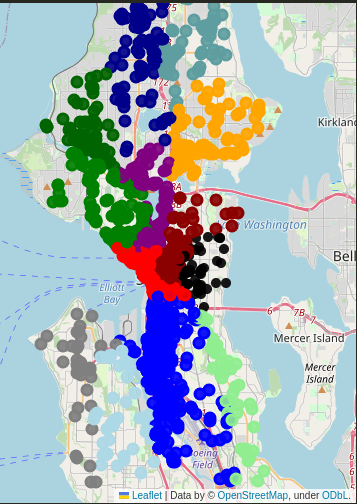
\includegraphics[height=30mm]{seattle_map.png}} ;
% 	\end{tikzpicture}

% \end{frame}

\begin{frame}[t, label=BaseDonnees]
	\vspace{0mm}
	\begin{tikzpicture}
		\linespread{1}% <--- locally defined vertical line spacing in nodes
		\draw[clrBorders] (0,0) rectangle (\txw,\txh) ;
		\nodePageNumber

		\node at (\midX,\midY) {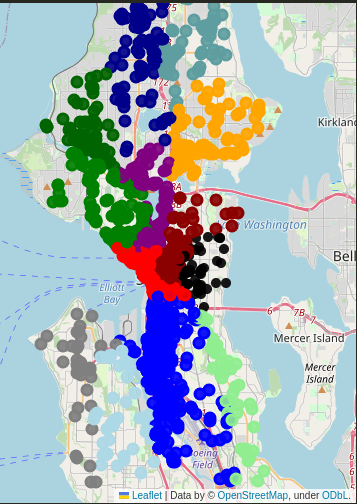
\includegraphics[height=55mm]{seattle_map.png}} ;

		\only<2->{
			\node[box_style00, text width=40mm] at (\midX,82mm) { 3376 entrées:\\1708 résidentielles\\\alert{1668 non résidentielles} } ;
		}

		\only<3->{
			\node[box_style00] at (\midX,13mm) {\alert{45 variables}} ;
		}

		\begin{scope}[xshift=15mm]
			\only<4->{ % IDENTIFICATION
				\node[box_style00, text=myOrng, text width=20mm] (IDsLoc) at (0,80mm) {Identification \& localisation} ;
				\begin{scope}[xshift=-10mm, yshift=74mm]
					\foreach \i/\x in {0/id, 1/nom , 2/adresse, 3/zipcode, 4/{...} }
					{
						\node[font=\fontsize{6}{6}\selectfont, anchor=west, text height=3mm]
							at (0,-\i*2.5mm) { $\bullet$ \x } ;
					}
				\end{scope}
			}

			\only<5->{ % DATES
				\begin{scope}[yshift=55mm]
					\node[box_style00, text=myOrng, text width=20mm] (Dates) at (0,0) {Dates} ;
					\begin{scope}[xshift=-10mm, yshift=-4mm]
						\foreach \i/\x in {0/date des données , 1/date de construction}
						{
							\node[font=\fontsize{6}{6}\selectfont, anchor=west, text height=3mm]
							at (0,-\i*2.5mm) { $\bullet$ \x } ;
						}
					\end{scope}
				\end{scope}
			}

			\only<6->{ % DIMENSIONS
				\begin{scope}[yshift=38mm]
					\node[box_style00, text=myOrng, text width=20mm] (Dates) at (0,0) {Dimensions} ;
					\begin{scope}[xshift=-10mm, yshift=-4mm]
						\foreach \i/\x in {0/nombre de bâtiments, 1/nombre de niveaux, 2/surface, 3/surface parking}
						{
							\node[font=\fontsize{6}{6}\selectfont, anchor=west, text height=3mm]
								at (0,-\i*2.5mm) { $\bullet$ \x } ;
						}
					\end{scope}
				\end{scope}
			}

			\only<7->{ % CERTIFICATION
				\begin{scope}[yshift=18mm]
					\node[box_style00, text=myOrng, text width=20mm] (Certif) at (0,0) {Certification} ;
					\begin{scope}[xshift=-10mm, yshift=-4mm]
						\foreach \i/\x in {0/EnergySTARSCORE, 1/dates de certification}
						{
							\node[font=\fontsize{6}{6}\selectfont, anchor=west, text height=3mm]
								at (0,-\i*2.5mm) { $\bullet$ \x } ;
						}
					\end{scope}
				\end{scope}
			}
		\end{scope}

		\begin{scope}[xshift=90mm]
			\only<8->{ % UTILISATIONS
				\begin{scope}[yshift=80mm]
					\node[box_style00, text=myOrng, text width=20mm] (Utilisation) at (0,0) {Utilisations} ;
					\begin{scope}[xshift=-10mm, yshift=-4mm]
						\foreach \i/\x in {0/type de propriété, 1/type de bâtiment, 2/utilisations principales, 3/surface par utilisation, 4/{...}}
						{
							\node[font=\fontsize{6}{6}\selectfont, anchor=west, text height=3mm]
								at (0,-\i*2.5mm) { $\bullet$ \x } ;
						}
					\end{scope}
				\end{scope}
			}

			\only<9->{ % ENERGIES
				\begin{scope}[yshift=52mm]
					\node[box_style00, text=myOrng, text width=20mm] (Utilisation) at (0,0) {Consommation\\\& émissions} ;
					\begin{scope}[xshift=-10mm, yshift=-6mm]
						\foreach \i/\x in {0/conso. {elec./gas/steam}, 1/consommation totale, 2/émissions totales, 3/{...}}
						{
							\node[font=\fontsize{6}{6}\selectfont, anchor=west, text height=3mm]
								at (0,-\i*2.5mm) { $\bullet$ \x } ;
						}
					\end{scope}
				\end{scope}
			}


			\only<10->{ % AUTRES
				\begin{scope}[yshift=25mm]
					\node[box_style00, text=myOrng, text width=20mm] (Utilisation) at (0,0) {Autres} ;
					\begin{scope}[xshift=-10mm, yshift=-4mm]
						\foreach \i/\x in {0/DefaultData, 1/ComplianceStatus, 2/Outlier}
						{
							\node[font=\fontsize{6}{6}\selectfont, anchor=west, text height=3mm]
								at (0,-\i*2.5mm) { $\bullet$ \x } ;
						}
					\end{scope}
				\end{scope}
			}

		\end{scope}

	\end{tikzpicture}
\end{frame}

\begin{frame}[t, label=objectif]
	\vspace{0mm}
	\begin{tikzpicture}
		\linespread{1}% <--- locally defined vertical line spacing in nodes
		\draw[clrBorders] (0,0) rectangle (\textwidth,\textheight) ;
		\nodePageNumber

		\begin{scope}[xshift=-5mm]
			\node at (22mm, 68mm) { Relevés } ;
			\node at (20mm,50mm) (A) {
\includegraphics[height=30mm]{mathafix-bourse.pdf}} ;

			\only<2->{
				\node[box_style00] (B) at (50mm, 50mm) { Modélisation } ;
				\draw[myarrow] (A) -- (B) ;
			}

			\only<3->{
				\node[box_style00] (C) at (80mm, 50mm) { Prédiction } ;
				\draw[myarrow] (B) -- (C) ;
			}

			\only<4->{
				\node[box_style00, text width=20mm] (Da) at (65mm,30mm) {\alert{Consommation} totale} ;
				\node[box_style00, text width=20mm] (Db) at (95mm,30mm) {\alert{Émissions} totales} ;
				\draw[myarrow] (C) -- ++ (0, -7mm) -| (Da) ;
				\draw[myarrow] (C) -- ++ (0, -7mm) -| (Db) ;
			}

			\only<5>{
				\node[box_style00, text = myOrng, font=\bfseries, text width=35mm] (E) at (50mm,75mm) {Intérêt\\EnergySTARSCORE ?} ;
				\draw[myarrow, myOrng] (E) -- (B) ;
			}
		\end{scope}
	\end{tikzpicture}
\end{frame}


\section{EXPLORATION DES DONNÉES \& DÉFINITION DES VARIABLES CIBLES}
\subsection{Épuration des données}

\begin{frame}[t, label=epuration]
	\vspace{0mm}
	\begin{tikzpicture}
		\linespread{1}% <--- locally defined vertical line spacing in nodes
		\draw[clrBorders] (0,0) rectangle (\textwidth,\textheight) ;
		\nodePageNumber


		\onlystyle<5->{removed}{myShaded}

		\node at (30mm,85mm) {Suppression des \alert{variables en double}:} ;
		\only<2->{
		\begin{scope}[xshift=10mm, yshift=75mm]
			\node[box_style00, anchor=west] at (0,0) {Électricité (kBtu)} ;
			\node[box_style00, anchor=west, removed] at (30mm,0) {Électricité (kWh)} ;
		\end{scope}}

		\only<3->{
		\begin{scope}[xshift=10mm, yshift=65mm]
			\node[box_style00, anchor=west] at (0,0) {Gas naturel (kBtu)} ;
			\node[box_style00, anchor=west, removed] at (30mm,0) {Gas naturel (therms)} ;
		\end{scope}}

		\only<4->{
			\node[box_style00, anchor=west] at (10mm,55mm) {Consommation totale (kBtu)} ;
		}

		\only<6->{
			\node at (30mm,43mm) {Suppression des \alert{entrées "invalides"}:} ;
		}
		\only<7->{
			\node at (\midX,20mm) {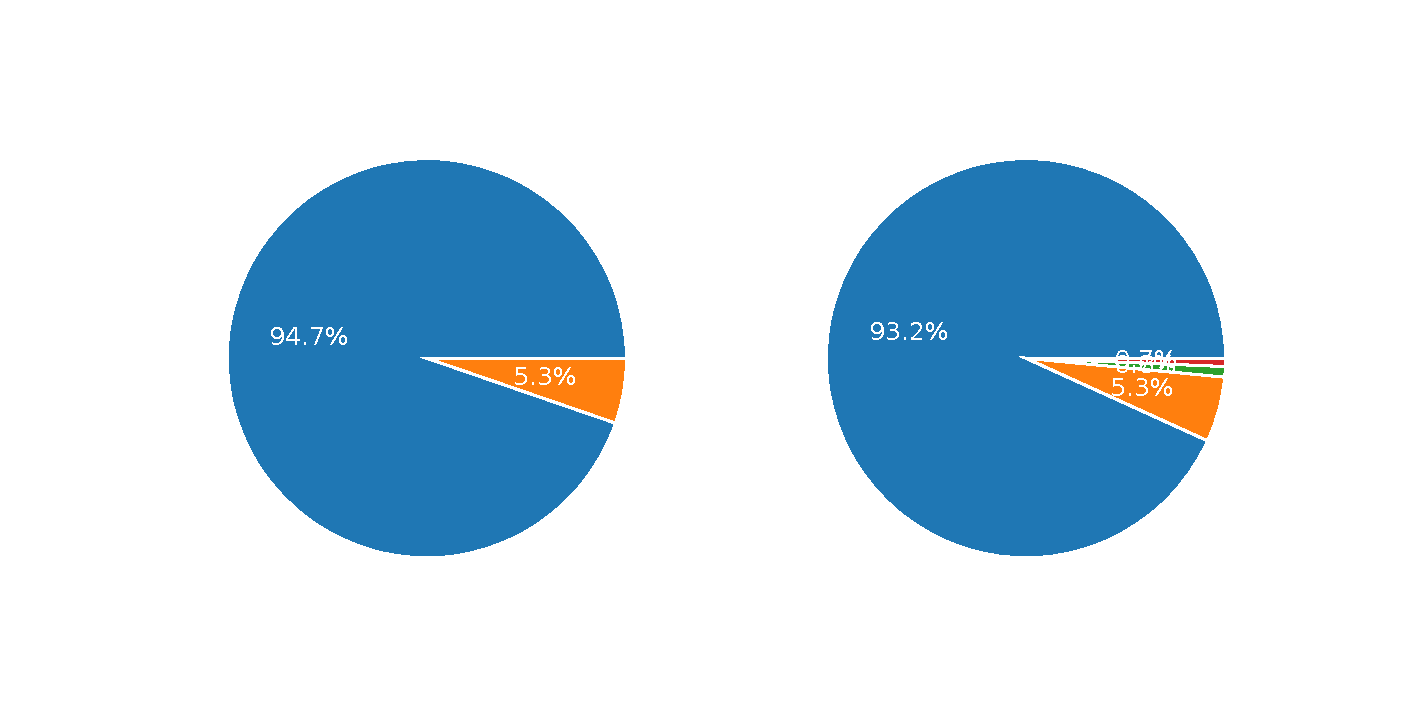
\includegraphics[width=90mm]{outliers_compliant.pdf}} ;
		}
	\end{tikzpicture}
\end{frame}

\subsection{Vérification des données}
\begin{frame}[t, label=verif]

	% VÉRIFICATION DES DONNÉES

	% graph surfaces -> on prend GFA Building(s)

	% graph energy / surface : -> à recalculer

	% graph histogrammes energy : lin / log \& total / surfacique

	% graph emissions : formule validée

	\vspace{0mm}
	\begin{tikzpicture}
		\linespread{1}% <--- locally defined vertical line spacing in nodes
		\draw[clrBorders] (0,0) rectangle (\textwidth,\textheight) ;
		\nodePageNumber

		\node at (35mm,\midY) {\includegraphics<1-2>[width=60mm]{verif_GFA.pdf}} ;
		\node at (35mm,\midY) {\includegraphics<3-4>[width=60mm]{verif_energies.pdf}} ;
		\node at (35mm,\midY) {\includegraphics<5-6>[width=60mm]{verif_siteEUI.pdf}} ;
		\node at (35mm,\midY+15mm) {\includegraphics<7-9>[width=60mm]{histo_SiteEnergyUseWN(kBtu)_log.pdf}} ;
		\node at (35mm,\midY-15mm) {\includegraphics<8-9>[width=60mm]{histo_Nrg_GFA_Buildings_log.pdf}} ;
		\node at (35mm,\midY) {\includegraphics<10-11>[width=60mm]{verif_emissions.pdf}} ;

		\onlystyle<2>{highlightGFA}{myOrng}
		\onlystyle<4>{highlightCONSO}{myOrng}
		\onlystyle<6>{highlightCONSO2}{myOrng}
		\onlystyle<9>{highlightTarget}{myOrng}
		\onlystyle<11>{highlightEmissions}{myOrng}

		\begin{scope}[yshift=-15mm]
			\only<2->{\node[box_style00, text width=30mm, highlightGFA] at (90mm, 85mm) {Référénce GFA Buidlings} ;}

			\only<4->{\node[box_style00, text width=30mm, highlightCONSO] at (90mm, 75mm) {Re-calcul consommation totale} ;}

			\only<6->{\node[box_style00, text width=30mm, highlightCONSO2] at (90mm, 65mm) {Re-calcul consommation surfacique} ;}

			\only<9->{\node[box_style00, text width=30mm, highlightTarget] at (90mm, 55mm) {Cible : consommation surfacique} ;}

			\only<11->{\node[box_style00, text width=30mm, highlightEmissions] at (90mm, 43mm) {Calcul des émissions à partir de la consommation} ;}

		\end{scope}

		% \node at (0.5\textwidth,0.5\textheight) {\includegraphics<10>[width=30mm]{histo_TotalGHGEmissions_log.pdf}} ;

		\only<13->{
			\node[box_style00, text width=40mm, text=myOrng] at (30mm,70.2mm) (cclA) {Nécessité de re-calculer des variables} ;
			\draw[myarrow] (70mm, 50mm) -- ++ (-7mm,0) |- (cclA) ;
		}
		\only<14->{
			\node[box_style00, text width=40mm, text=myOrng, below=of cclA, yshift=4.1mm] (cclB) {Utilisation des valeurs "Weather Normalized"} ;
			\draw[myarrow] (70mm, 50mm) -- ++ (-7mm,0) |- (cclB) ;
		}
		\only<15->{
			\node[box_style00, text width=40mm, text=myOrng, below=of cclB, yshift=4.1mm] (cclC) {Modélisation de la consommation surfacique} ;
			\draw[myarrow] (70mm, 50mm) -- ++ (-7mm,0) |- (cclC) ;
		}
		\only<16->{
			\node[box_style00, text width=40mm, text=myOrng, below=of cclC, yshift=4.1mm] (cclD) {Prédiction des émissions à partir des prédictions sur la consommation} ;
			\draw[myarrow] (70mm, 50mm) -- ++ (-7mm,0) |- (cclD) ;
		}

		\only<12->{
			\draw[line width=0.7mm] (70mm, 23mm) -- ++ (0, 50mm) ;
		}
	\end{tikzpicture}
\end{frame}


% \begin{frame}[t, label=ccltarget]

% 	CONCLUSION EXPLORATION

% 	cible modèles : consommation par unité de surface (Weather Normalized)

% 	puis calcul de la valeur totale

% 	finalement calcul des émissions à partir de la consommation et des proportions d'énergies utilisées
% 	\vspace{0mm}
% 	\begin{tikzpicture}
% 		\linespread{1}% <--- locally defined vertical line spacing in nodes
% 		\draw[clrBorders] (0,0) rectangle (\textwidth,\textheight) ;

% 		\node at (0.2\textwidth,0.8\textheight) {\includegraphics<1>[width=40mm]{verif_nrgUseWN.pdf}} ;


% 	\end{tikzpicture}
% \end{frame}


\section{FEATURE ENGINEERING}

\subsection{Corrélation des variables initiales}
\begin{frame}[t, label=correlationInit]
	\vspace{0mm}
	\begin{tikzpicture}
		\linespread{1}% <--- locally defined vertical line spacing in nodes
		\draw[clrBorders] (0,0) rectangle (\textwidth,\textheight) ;
		\nodePageNumber

		\only<1>{
			\node at (\midX,\midY){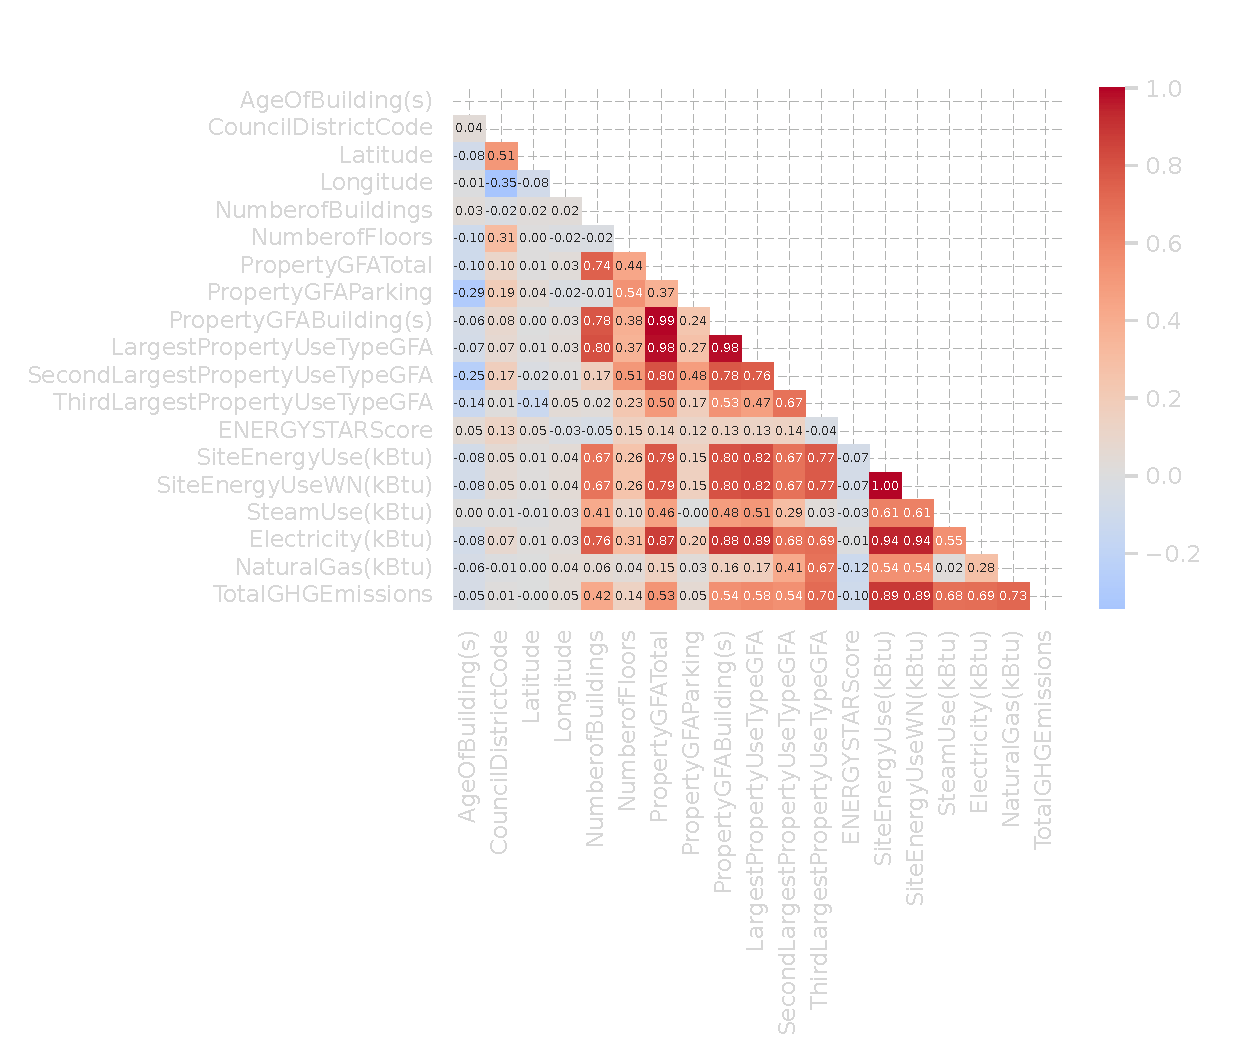
\includegraphics[width=100mm]{correl_init.pdf}} ;
		}

		\only<2->{
			\only<3>{
				\node at (\midX,20mm) {Présence de \alert{fortes multi-colinéarités}} ;
			}
		\node at (\midX, 65mm) { Multi-colinéarité (Variance Inflation Factor)} ;
		\node at (\midX,\midY){ \small
		\begin{tabular}{ccc}
			\rowcolor{dfFirstRow}
			 & feature & VIF \tabularnewline
			\rowcolor{dfEvenRow}
			4 & NumberofBuildings & 113400533.76 \tabularnewline
			\rowcolor{dfOddRow}
			6 & PropertyGFATotal & inf \tabularnewline
			\rowcolor{dfEvenRow}
			7 & PropertyGFAParking & inf \tabularnewline
			\rowcolor{dfOddRow}
			8 & PropertyGFABuilding(s) & inf \tabularnewline
			\rowcolor{dfEvenRow}
			9 & LargestPropertyUseTypeGFA & 30.29 \tabularnewline
			\rowcolor{dfOddRow}
			10 & SecondLargestPropertyUseTypeGFA & 5.9 \tabularnewline
			\rowcolor{dfEvenRow}
			11 & ThirdLargestPropertyUseTypeGFA & 6.29 \tabularnewline
			\rowcolor{dfOddRow}
			14 & Electricity(kBtu) & 5.85 \tabularnewline
			\rowcolor{dfEvenRow}
			15 & NaturalGas(kBtu) & 5.52
		\end{tabular}
		} ; }
	\end{tikzpicture}
\end{frame}

\subsection{Analyse en Composantes Principales}
\begin{frame}[t, label=PCA]
	\vspace{0mm}
	\begin{tikzpicture}
		\linespread{1}% <--- locally defined vertical line spacing in nodes
		\draw[clrBorders] (0,0) rectangle (\textwidth,\textheight) ;
		\nodePageNumber

		\node at (\midX,\midY) {\includegraphics<1-2>[width=90mm]{PCA_eboulis.pdf}} ;
		\only<2>{
			\node[myOrng, font=\bfseries, text width = 17mm, text centered]
				(A) at (68.5mm, 50.5mm) { $\ge$ 90\% pour\\8 variables } ;
			\draw[myarrow, myOrng] (A.north west) -- ++ (-10mm,5.8mm) ;
		}
		\node at (\midX+6mm,\midY-8mm) {\includegraphics<3>[width=100mm]{PCA_heatmap.pdf}} ;
		\only<3>{
			\node at (\midX,72mm) {Projection des variables sur les principaux axes d'inertie:} ;
		}

	\end{tikzpicture}
\end{frame}

\subsection{Type d'énergies consommées}
\begin{frame}[t, label=propNrj]
	\vspace{0mm}
	\begin{tikzpicture}
		\linespread{1}% <--- locally defined vertical line spacing in nodes
		\draw[clrBorders] (0,0) rectangle (\textwidth,\textheight) ;
		\nodePageNumber

		\node[box_style00, text width=25mm] at (22mm,62mm) {\alert{Corrélation importante}\\entre la {consommation totale} et la {consommation élec./gas/vapeur}\\(54\% à 96\%)} ;
		\only<2->{*
			\node[box_style00, text width=25mm] at (22mm, 33mm) {Des \alert{ratios} sont calculés pour éviter la \alert{fuite de données} : valeurs normalisées par la consommation totale} ;
		}
		\only<3>{
			\node at (\midX+20mm,\midY) {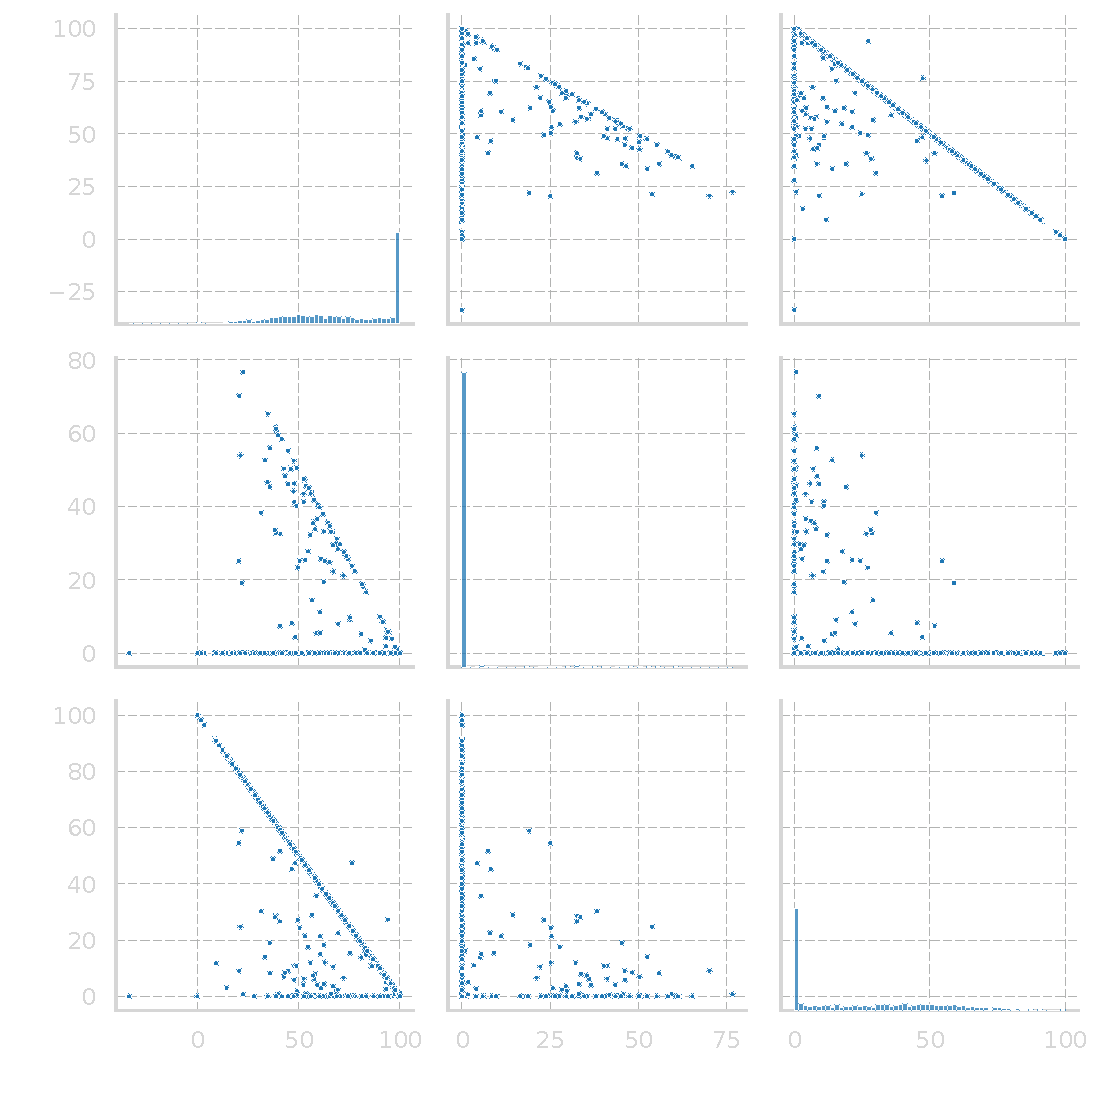
\includegraphics[width=60mm]{prop_energies.pdf}} ;
		}
	\end{tikzpicture}
\end{frame}

\subsection{Surfaces et types d'utilisations}
\begin{frame}[t, label=oheUseTypeGFA]
	% CATEGORIES / ONE HOT ENCODING

	% 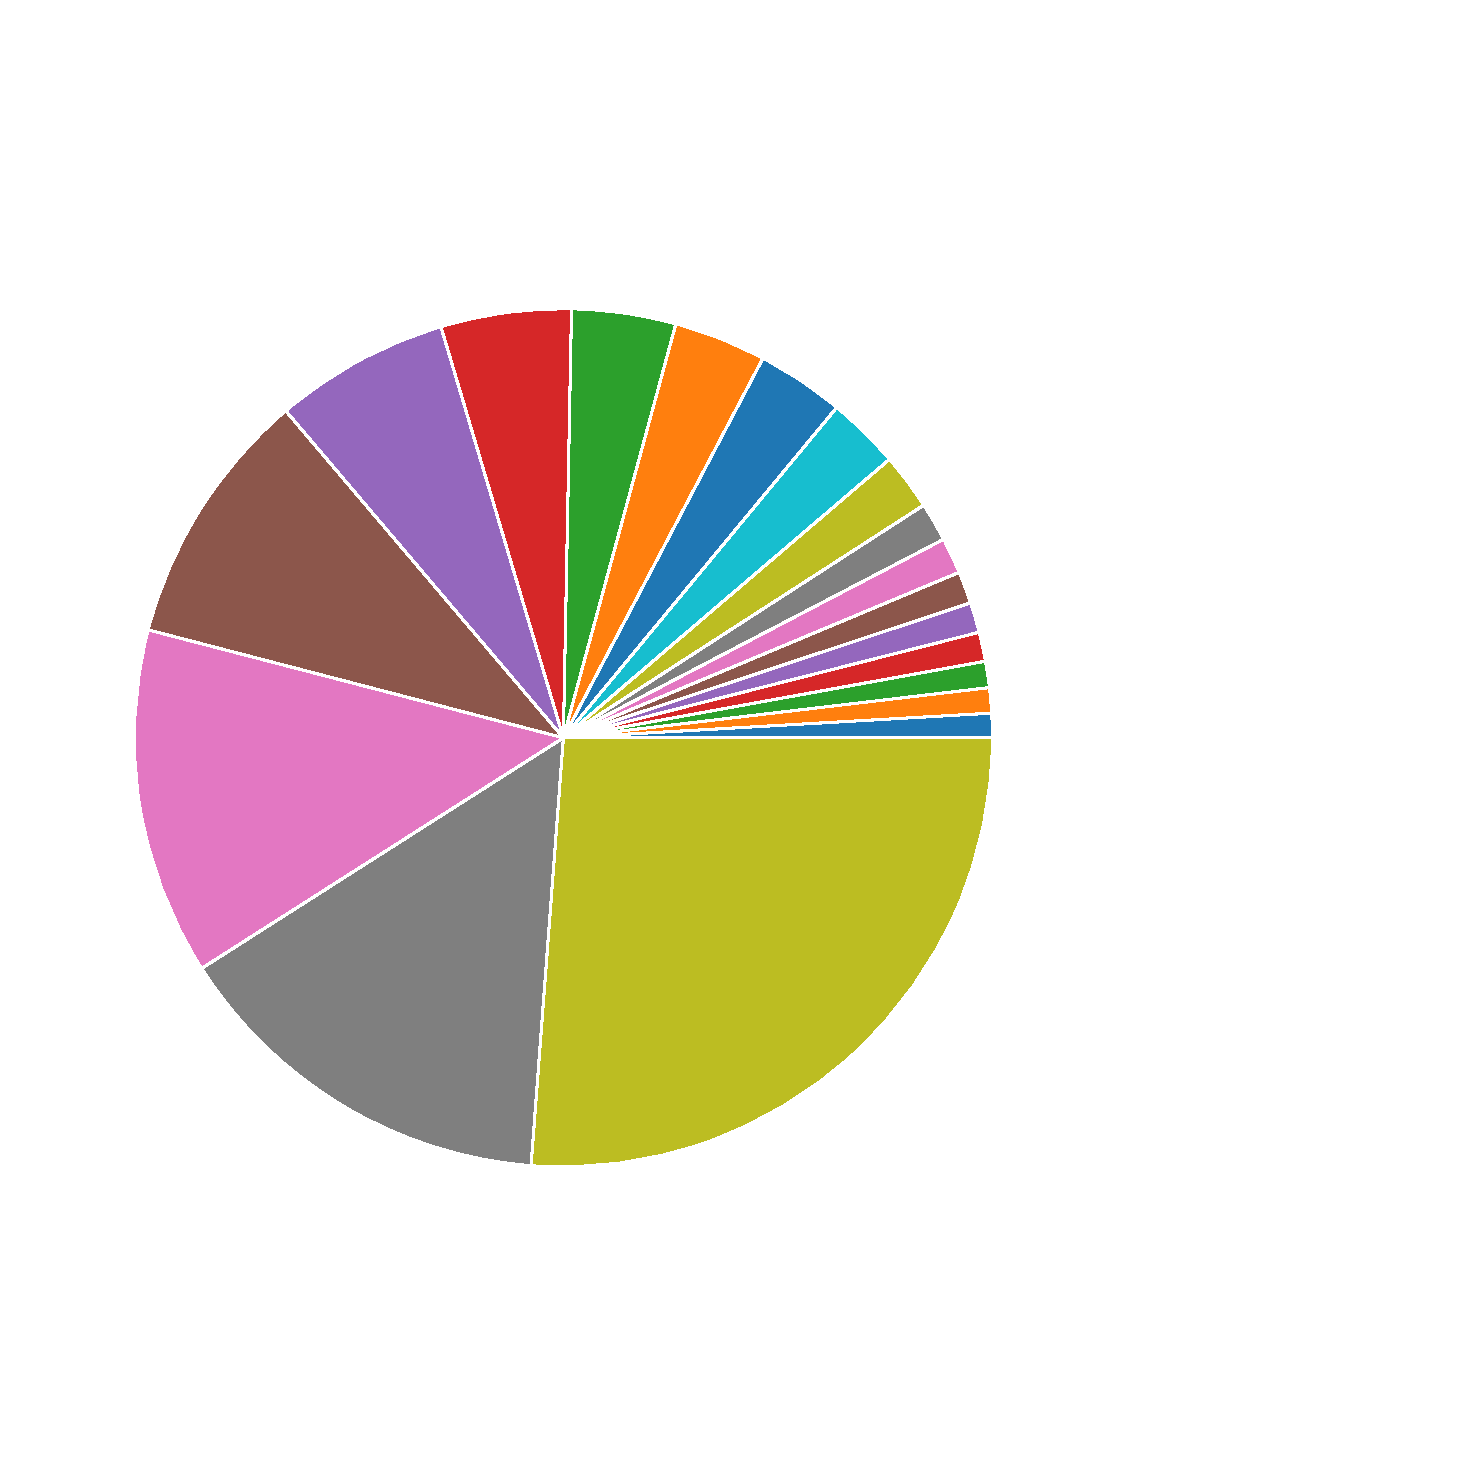
\includegraphics[width=30mm]{categories.pdf}

	% 1$^{er}$, 2$^{ème}$ et 3$^{ème}$ PropertyUseType $\rightarrow$ 63 catérgories classées en 19 catégories

	% les données sont coder selon un schéma OneHotEncoding, (19 colonnes / 1 par catégorie), avec comme poids les
	% 1$^{er}$, 2$^{ème}$ et 3$^{ème}$ PropertyUseTypeGFA


	\vspace{0mm}
	\begin{tikzpicture}
		\linespread{1}% <--- locally defined vertical line spacing in nodes
		\draw[clrBorders] (0,0) rectangle (\textwidth,\textheight) ;
		\nodePageNumber

		\node[anchor=west, text width=60mm] (A) at (\midX-31.3mm, 80mm) {Données initiales:\\ \hspace{2mm}$\bullet$ 3 premières utilisations principales\\ \hspace{2mm}$\bullet$ 63 catégories} ;

		\only<2->{
			\node[below=of A, yshift=3mm] (B) {\alert{Re-classement en 19 catégories}} ;
			\draw[myarrow] (A) -- (B) ;
		}
		\only<3>{
			\node at (60mm,33mm) {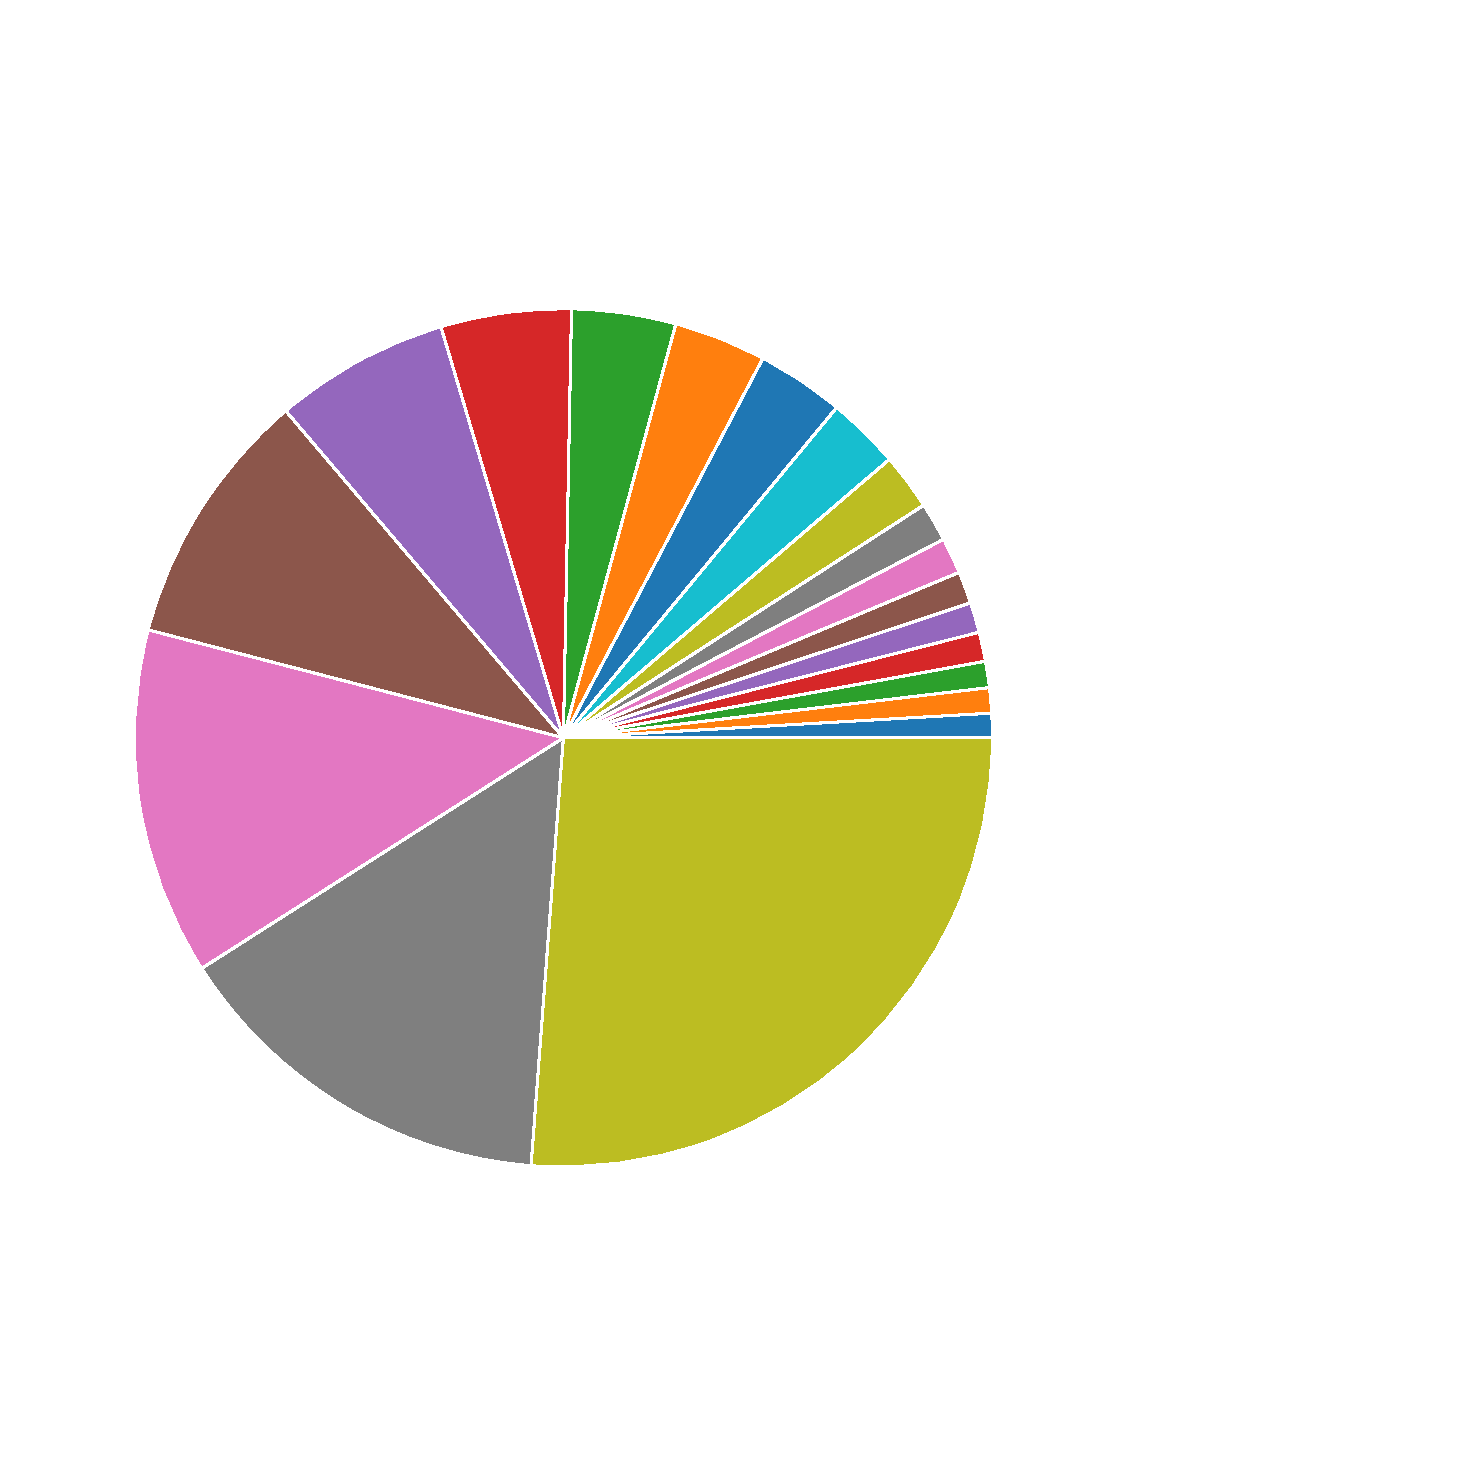
\includegraphics[width=75mm]{categories.pdf}} ;
		}

		\only<4->{
			\node[text centered, text width = 80mm] (C) at (\midX,50mm) {Codé selon la méthode "\alert{One Hot Encoding}"\\\alert{Surfaces normalisées} par le "GFA Building(s)"} ;
			\draw[myarrow] (B) -- (C) ;
		}

		\only<5>{
			\node at (\midX,25mm) {\begin{tabular}{>{\centering}m{5mm}>{\centering}m{15mm}>{\centering}m{15mm}>{\centering}m{15mm}>{\centering}m{15mm}>{\centering}m{15mm}}
				\rowcolor{dfFirstRow}
				& ohe0 data center & ohe0 education & ohe0 entertainment - public assembly & ohe0 industrial & ohe0 lifestyle center \tabularnewline
				\rowcolor{dfEvenRow}
				16 & 0.0 & 0.0 & 0.0 & 0.0 & 0.87 \tabularnewline
				\rowcolor{dfOddRow}
				17 & 0.0 & 0.0 & 0.0 & 0.0 & 0.0 \tabularnewline
				\rowcolor{dfEvenRow}
				18 & 0.0 & 0.0 & 0.29 & 0.0 & 0.0 \tabularnewline
				\rowcolor{dfOddRow}
				19 & 0.0 & 0.0 & 0.0 & 0.0 & 0.0 \tabularnewline
				\rowcolor{dfEvenRow}
				20 & 0.0 & 0.0 & 0.0 & 0.0 & 0.0
			\end{tabular}} ;
		}
	\end{tikzpicture}
\end{frame}


\subsection{Nouvelles variables}
\begin{frame}[t, label=NewVars]
	% NOUVELLES VARIABLES

	% données temporelles : YearBuilt et DataYear

	% création d'une nouvelle variable : Age du bâtiment ( DataYear - YearBuilt )

	% suppression de YearBuilt et DataYear


	% \alert{variables liées à l'équation de transfers thermiques:}\\
	% GFA per floor = GFA building(s) / (number of buildings * number of floors)
	% \\
	% $\sqrt{GFA per floor}$ : approximation du périmètre (Surface d'échange / hauteur supposée normalisée)

	\vspace{0mm}
	\begin{tikzpicture}
		\linespread{1}% <--- locally defined vertical line spacing in nodes
		\draw[clrBorders] (0,0) rectangle (\textwidth,\textheight) ;
		\nodePageNumber

		\begin{scope}[xshift=5mm, yshift=5mm]
			\node[anchor=west] at (0mm,80mm) {Données \alert{temporelles}:} ;
			\only<2->{
				\node[box_style00, text width=16mm] (DataYear) at (20mm,70mm) {Date des données} ;
				\node[box_style00, text width=16mm, below=of DataYear, yshift=5mm] (YearBuilt) {Date de construction} ;
			}
			\only<3->{
				\node[draw, circle] (SUB) at (45mm, 63.8mm) {-} ;
				\draw[myarrow] (DataYear.east) -| (SUB) ;
				\draw[myarrow] (YearBuilt.east) -| (SUB) ;
			}
			\only<4->{
				\node[box_style00, text width=16mm, right=of SUB] (Age) {Âge du bâtiment} ;
				\draw[myarrow] (SUB) -- (Age) ;
			}
		\end{scope}

		\onlystyle<14->{highlight}{myOrng}
		\begin{scope}[yshift=10mm]
			\only<5->{
				\node[anchor=west] at (5mm, 40mm) {Variables liées à l'équation de \alert{transferts thermiques}:} ;
			}

			\visible<7->{
				\node[draw, circle] (mult) at (34mm,30mm) {$\times$} ;
			}
			\visible<6->{
				\node[box_style00, text width=16mm, left=of mult, xshift=3mm] (NB) {Nombre de bâtiments} ;
				\node[box_style00, text width=16mm, right=of mult, xshift=-3mm] (NF) {Nombre de niveaux} ;
			}
				
			\visible<8->{
				\node[box_style00, text width=16mm, below=of mult, yshift=3mm] (NTF) {Nombre total de niveaux} ;
				\draw[myarrow] (mult) -- (NTF) ;
			}

			\visible<7->{
			\draw[myarrow] (NB) -- (mult) ;
			\draw[myarrow] (NF) -- (mult) ;
			}

			\visible<10->{
				\node[draw, circle, right=of NTF, xshift=-3mm] (div) {/} ;
			}
			\visible<9->{
				\node[box_style00, text width=16mm, right=of div, xshift=-3mm] (GFA) {Surface bâtiments} ;
			}

			\visible<10->{
				\draw[myarrow] (NTF) -- (div) ;
				\draw[myarrow] (GFA) -- (div) ;
			}

			\visible<11->{
				\node[box_style00, text width=16mm, below=of div, yshift=3mm, highlight] (GFAPerFloor) {GFA par niveau} ;
				\draw[myarrow] (div) -- (GFAPerFloor) ;
			}

			

			\visible<12->{
				\node[draw, circle, right=of GFAPerFloor, xshift=-3mm] (SQRT) {$\sqrt{\phantom{a}}$} ;
				\draw[myarrow] (GFAPerFloor) -- (SQRT) ;
			}
			\visible<13->{
				\node[box_style00, text width=16mm, right=of SQRT, xshift=-3mm, highlight] (Perimeter) {Approx. périmètre} ;
				\draw[myarrow] (SQRT) -- (Perimeter) ;
			}
		\end{scope}

	\end{tikzpicture}
\end{frame}


\subsection{Corrélation des nouvelles variables}
\begin{frame}[t, label=correlationEngineeredFeatures]

	% graph: corrélations linéaires

	% vif : tableau

	% CCL : améliorations par rapport aux variables initiales

	\vspace{0mm}
	\begin{tikzpicture}
		\linespread{1}% <--- locally defined vertical line spacing in nodes
		\draw[clrBorders] (0,0) rectangle (\textwidth,\textheight) ;
		\nodePageNumber
		\only<1>{
			\node at (\midX,\midY){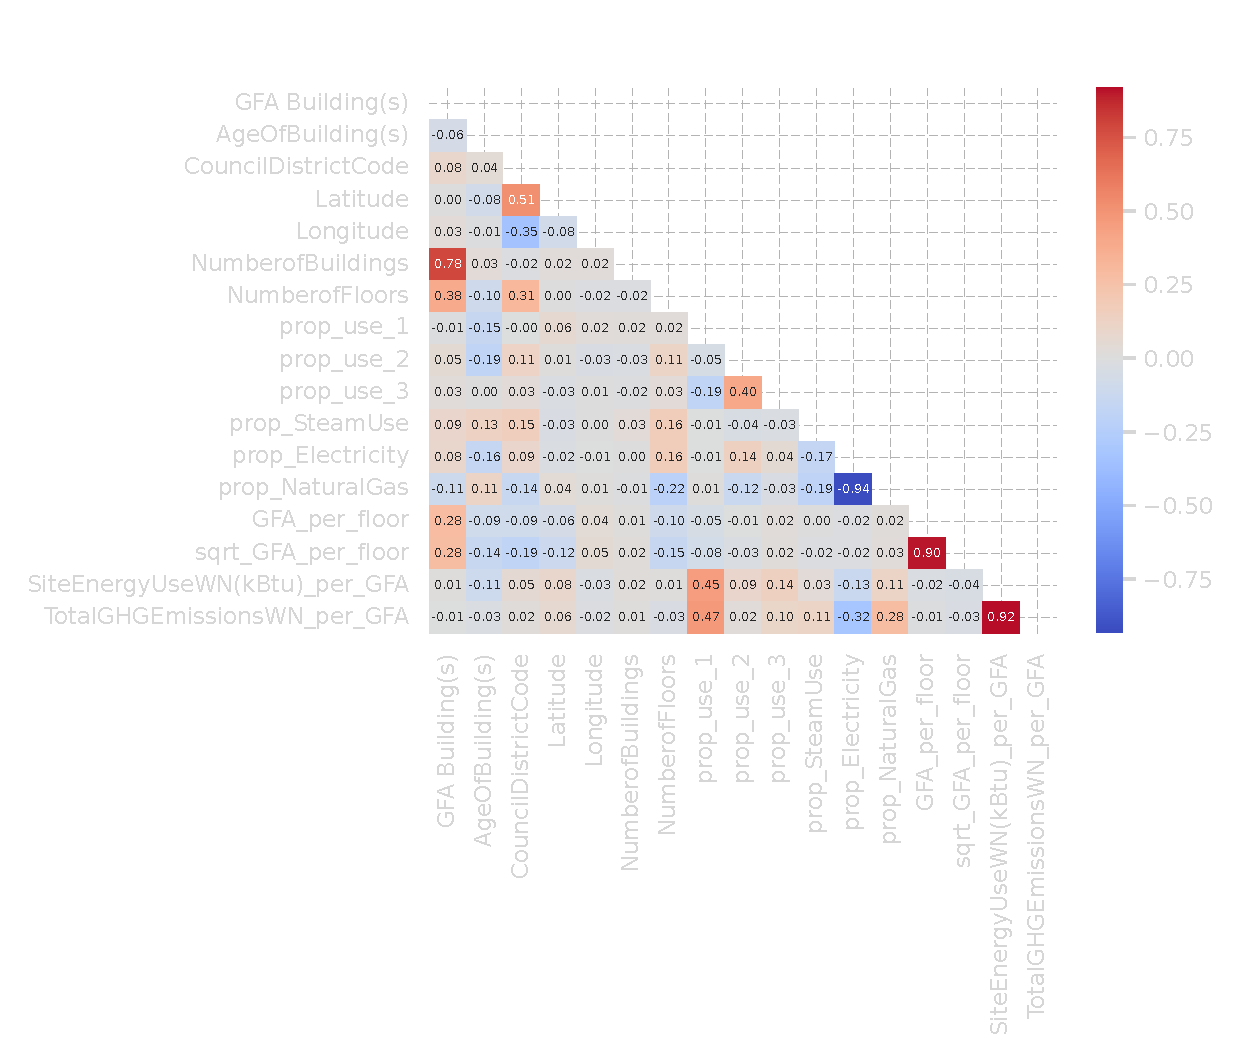
\includegraphics[width=100mm]{correl_engineered.pdf}} ;
		}

		\only<3>{
			\node at (\midX,20mm) {Diminution des \alert{multi-colinéarités}} ;
		}
		\only<2->{
		\node at (\midX, 65mm) { Multi-colinéarité (Variance Inflation Factor)} ;
		\node at (\midX,\midY){
			\begin{tabular}{ccc}
			\rowcolor{dfFirstRow}
			 & feature & VIF \tabularnewline
			\rowcolor{dfEvenRow}
			1 & CouncilDistrictCode & 7.73 \tabularnewline
			\rowcolor{dfOddRow}
			2 & Latitude & 1375267.78 \tabularnewline
			\rowcolor{dfEvenRow}
			3 & Longitude & 1374688.07 \tabularnewline
			\rowcolor{dfOddRow}
			6 & prop use 1 & 6.12 \tabularnewline
			\rowcolor{dfEvenRow}
			10 & prop Electricity & 164.76 \tabularnewline
			\rowcolor{dfOddRow}
			11 & prop NaturalGas & 43.07 \tabularnewline
			\rowcolor{dfEvenRow}
			12 & GFA per floor & 7.12 \tabularnewline
			\rowcolor{dfOddRow}
			13 & sqrt GFA per floor & 27.53
		\end{tabular}} ;
		}
	\end{tikzpicture}
\end{frame}



\section{MODÉLISATION}
\subsection{Consommation d'énergie}

\begin{frame}[t, label=ModelProcessus]
	\vspace{0mm}
	\begin{tikzpicture}
		\linespread{1}% <--- locally defined vertical line spacing in nodes
		\draw[clrBorders] (0,0) rectangle (\textwidth,\textheight) ;
		\nodePageNumber

		\onlystyle<13->{highlight}{myOrng}
		\tikzset{donnes/.style = {cyan}}

		\visible<13>{
			\node[box_style00, myOrng, text width = 25mm] at (16mm,50mm) {2 étapes\\optionnelles\\{\large $\downarrow$}\\4 configurations} ;
		}

		\visible<5->{
		\node[box_style00] (B) at (36mm,0.7\textheight) {Grid search CV} ;
		}
		\visible<2->{
		\node[box_style00, text width=20mm, above=of B, highlight] (AaScale) {Mise à l'échelle} ;
		}

		\node[box_style00, left=of AaScale, donnes] (Aa) {$X_{train}$} ;


		\visible<4->{
		\node[draw, circle, below=of B, highlight] (LOG) {log} ;
		\node[draw, circle, below=of LOG] (Ad) {/} ;
		}
		\visible<3->{
		\node[box_style00, left=of Ad, donnes] (Ab) { $y_{train}$} ;
		\node[box_style00, below=of Ab, yshift=5mm, donnes] (Ac) { $GFA_{train}$} ;
		}
		% \begin{scope}[xshift=0.15\textwidth, yshift=0.5\textheight]
		% 	\node[box_style00, text width=20mm] (Ab) at (0,0) { $y_{train}$} ;
		% 	\node[box_style00, text width=20mm] (Ac) at (0,-7mm) { $GFA_{train}$} ;

		% 	\node[draw, circle] (Ad) at (20mm, 0) {div} ;
		% \end{scope}

		\visible<6->{
		\node[box_style00, right=of B, xshift=15mm] (Model) {Modèle} ;
		}
		\visible<7->{
		\node[box_style00, above=of Model, highlight] (ScaleTest) {Mise à l'échelle} ;
		\node[box_style00, right=of ScaleTest, donnes] (Xtest) {$X_{test}$} ;
		}

		\visible<8->{
		\node[box_style00, below=of Model] (Pred) {Prédiction} ;
		\node[draw, circle, below=of Pred, yshift=3mm, highlight] (logInv) {exp} ;
		}
		\visible<9->{
		\node[box_style00, left=of Pred, xshift=5mm, donnes] (E) {$GFA_{test}$} ;
		}
		\visible<10->{
		\node[draw, circle, below=of logInv, yshift=3mm] (Mult) {$\times$} ;
		}
		\visible<11->{
		\node[box_style00, right=of Pred, xshift=-2mm, donnes] (G) {$y_{test}$} ;
		}
		\visible<12->{
		\node[box_style00, below=of Mult] (F) {Calcul de l'erreur} ;
		}
		\visible<4->{
		\draw[myarrow] (Ad.north) -- (LOG) ;
		\draw[myarrow] (Ab.east) -- (Ad) ;
		\draw[myarrow] (Ac.east) -| (Ad) ;
		}
		\visible<5->{
		\draw[myarrow] (LOG.north) -- (B) ;
		\draw[myarrow] (AaScale) -- (B) ;
		}
		\visible<2->{
		\draw[myarrow] (Aa) -- (AaScale) ;}

		\visible<6->{
		\draw[myarrow] (B) -- (Model) ;
		}
		\visible<7->{
		\draw[myarrow] (Xtest) -- (ScaleTest) ;
		\draw[myarrow] (ScaleTest) -- (Model) ;
		}
		\visible<8->{
		\draw[myarrow] (Model) -- (Pred) ;
		\draw[myarrow] (Pred) -- (logInv) ;
		}
		\visible<10->{logInv
		\draw[myarrow] (logInv) -- (Mult) ;
		\draw[myarrow] (E) |- (Mult) ;
		}
		\visible<12->{
		\draw[myarrow] (Mult) -- (F) ;
		\draw[myarrow] (G) |- (F) ;
		}
	\end{tikzpicture}
\end{frame}

\begin{frame}[t, label=modelesDefinitions]

	% DummyRegressor: strategy

    % elastic net: l1\_ratio , alpha

    % linear SVR: loss , C

	% kernel ridge polynomial: alpha, degree = [1,2,3,4]

	% kernel ridge rbf: alpha , gamma

	% kernel SVR rbf: C , gamma

	% random forest: n\_estimators, min\_samples\_split, max\_depth, max\_features

	% light GBM:  n\_estimators, subsample, learning\_rate, max\_depth

	\vspace{0mm}
	\begin{tikzpicture}
		\linespread{1}% <--- locally defined vertical line spacing in nodes
		\draw[clrBorders] (0,0) rectangle (\textwidth,\textheight) ;
		\nodePageNumber

		\begin{scope}[xshift=\midX, yshift=\midY]
			\node at (0,0) {8 modèles} ;
			% \foreach \i in {0,1,2,3,4,5,6,7}{
			% 	\dr
			% }
			\newdimen\R
   			\R=14mm
			\draw[thick, myOrng] (22.5:\R) \foreach \x in {45,90,...,360} {  -- (22.5+\x:\R) };
		\end{scope}

		\begin{scope}[xshift=\midX, yshift=\midY]
			\foreach \i/\ii/\x in {0/2/dummy regressor, 1/3/{elastic\\net}, 2/4/{linear\\SVR}, 3/5/kernel ridge poly., 4/6/kernel ridge rbf, 5/7/kernel SVR rbf, 6/8/random forest, 7/9/{light\\GBM}}
			{
				\visible<\ii->{
					% \node[draw, circle, text centered, text width=15mm] at ( {29mm*sin(360*\i/8)}, {29mm*cos(360*\i/8)} ) {\x} ;
					\node[draw, circle, text centered, text width=15mm, text=myOrng] at ( 90-\i*45:29mm ) {\x} ;
				}
			}

			\visible<10->{
				\node[font=\itshape\small] at (90:42mm) {strategy} ;
			}
			\visible<11->{
				\node[font=\itshape\small, text width=10mm] at (45:45mm) {l1\_ratio\\alpha} ;
			}
			\visible<12->{
				\node[font=\itshape\small, text width=10mm] at (0:45mm) {loss\\C} ;
			}
			\visible<13->{
				\node[font=\itshape\small, text width=10mm] at (-45:45mm) {degree\\alpha} ;
			}
			\visible<14->{
				\node[font=\itshape\small, text width=10mm] at (-90:42mm) {gamma\\alpha} ;
			}
			\visible<15->{
				\node[font=\itshape\small, text width=10mm] at (-135:45mm) {gamma\\C} ;
			}
			\visible<16->{
				\node[font=\itshape\small, text width=10mm] at (-166:49mm) {n\_estimators\\min\_samples\_split\\max\_depth\\max\_features} ;
			}
			\visible<17->{
				\node[font=\itshape\small, text width=10mm] at (-210:49mm) {n\_estimators\\subsample\\learning\_rate\\max\_depth} ;
			}
		\end{scope}


	\end{tikzpicture}
\end{frame}


\begin{frame}[t, label=ResultsConso]

	% graph: results

	% random forest bien mais long

	% Kernel SVR rbf bien, rapide

	\vspace{0mm}
	\begin{tikzpicture}
		\linespread{1}% <--- locally defined vertical line spacing in nodes
		\draw[clrBorders] (0,0) rectangle (\textwidth,\textheight) ;
		\nodePageNumber

		\node at (\midX,70mm) {Résultats} ;
		\node at (\midX,\midY) {\includegraphics<1>[width=90mm]{results_conso.pdf}} ;

		\visible<2->{
		\node[fill=black!85, rounded corners] at (\midX,\midY) {\includegraphics<2>[width=90mm]{results_conso/dummy_median.pdf}} ;
		\node[fill=black!85, rounded corners] at (\midX,\midY) {\includegraphics<3>[width=90mm]{results_conso/kernel_SVR_rbf.pdf}} ;
		\node[fill=black!85, rounded corners] at (\midX,\midY) {\includegraphics<4>[width=90mm]{results_conso/random_forest.pdf}} ;
		}
	\end{tikzpicture}
\end{frame}


\begin{frame}[t, label=SHAP]

	% inflence des paramètres pour un outlier (consommation / GFA)

	% graph : shap outlier (kernel SVR rbf)

	% graph : feature importance (random forest)

	\vspace{0mm}
	\begin{tikzpicture}
		\linespread{1}% <--- locally defined vertical line spacing in nodes
		\draw[clrBorders] (0,0) rectangle (\textwidth,\textheight) ;
		\nodePageNumber

		\begin{scope}[yshift=0mm]
			\node at (\midX,85mm) {\alert{SHAP} pour un outlier (kernel SVR rbf)} ;
			\node at (\midX,0.8\textheight) {\includegraphics<2->[width=80mm]{SHAP_outlier.png}} ;
		\end{scope}

		\begin{scope}[yshift=-5mm]
			\visible<3->{
			\node at (0.8\textwidth,0.58\textheight) {Random forest} ;
			\node at (0.7\textwidth,0.4\textheight) {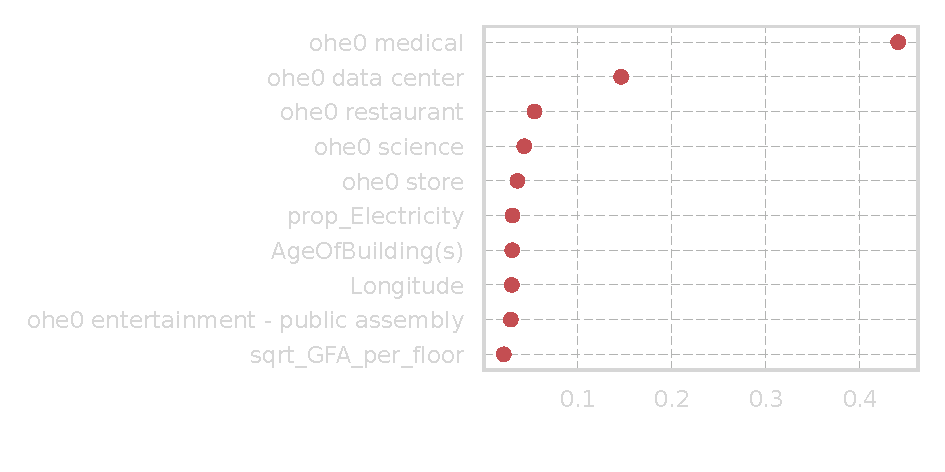
\includegraphics[width=60mm]{feature_importance.pdf}} ;
			}
			\begin{scope}[xshift=30mm, yshift=0.5\textheight]
				\node at (0,0) {\includegraphics<4->[width=50mm]{categories.pdf} } ;
				\visible<5->{
				\begin{scope}[ xshift=2mm, yshift=4.6mm]
					\begin{scope}[rotate=30]
						\draw[very thick, red] circle [x radius=8mm, y radius=1mm] ;
					\end{scope}
				\end{scope}}
			\end{scope}
			\visible<5->{
			\draw[myarrow, red] (43mm, 53mm) -- (65mm, 49.5mm) ;
			}
		\end{scope}

		\visible<6>{
			\node[box_style00, text width=50mm] at (\midX,10mm) {\alert{Impact conséquent d'outliers} (consommation surfacique)} ;
		}
	\end{tikzpicture}
\end{frame}

\subsection{Consommation sans outliers}
\begin{frame}[t, label=ConsoSansOutliers]
	\vspace{0mm}
	\begin{tikzpicture}
		\linespread{1}% <--- locally defined vertical line spacing in nodes
		\draw[clrBorders] (0,0) rectangle (\textwidth,\textheight) ;
		\nodePageNumber

		\node at (\midX,70mm) {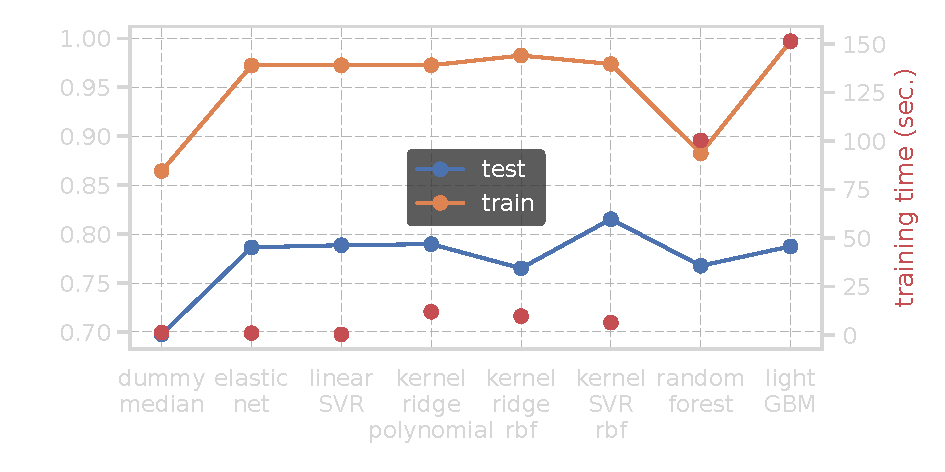
\includegraphics[width=80mm]{results_conso_without_outliers.pdf}} ;
		\visible<2->{
			\begin{scope}[xshift=63.1mm,yshift=61mm]
				\draw[rounded corners, myOrng, thick] (0,0) rectangle (5mm,25mm) ;
			\end{scope}
			\node[myOrng, text width=12mm] at (95mm,55mm) {Pertinent et rapide} ;
		}

		\visible<3->{
		\node at (\midX,43mm) {Light GBM} ;
		\node at (\midX,22mm) {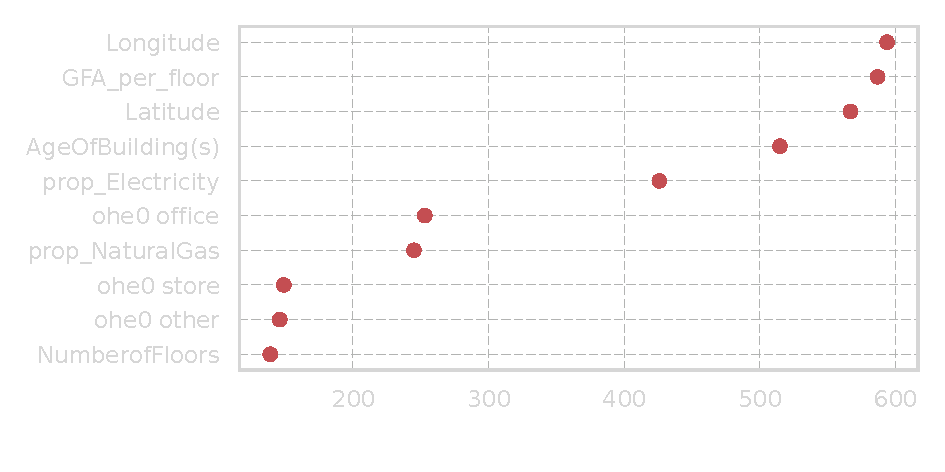
\includegraphics[width=80mm]{feature_importance_without_outliers.pdf}} ;
		}
		\visible<4>{
			\node[myOrng] at (68mm,16.2mm) {Répartition plus cohérente} ;
		}
	\end{tikzpicture}
\end{frame}

\subsection{Intérêt de l'EnergySTARSCORE}
\begin{frame}[t, label=EnergySTARSCORE]

	% kernel SVR rbf (R2 score train/test) : 0.97/0.82 $\rightarrow$ 0.96 / 0.94

	% intéressant, améliore les résultats mais coûteux à calculer.

	% Attention: le nombre de variables est réduit.

	% 1400 à 930 entrées
	\vspace{0mm}
	\begin{tikzpicture}
		\linespread{1}% <--- locally defined vertical line spacing in nodes
		\draw[clrBorders] (0,0) rectangle (\textwidth,\textheight) ;
		\nodePageNumber

		\node at (\midX,70mm) {R2 score kernel SVR rbf} ;
		\visible<2->{
		\node at (\midX,55mm) {
			\begin{tabular}{ccc}
				\rowcolor{dfFirstRow}
				EnergySTARSCORE & Sans  & Avec \tabularnewline
				\rowcolor{dfEvenRow}
				train set & 0.91 & 0.96 \tabularnewline
				\rowcolor{dfOddRow}
				test set & 0.92 & 0.94 \tabularnewline
				% \rowcolor{dfEvenRow}
				% nombre d'entrées & 1400 & 930
			\end{tabular}
		} ;}

		\visible<3->{
		\node[text width = 65mm, text centered] at (\midX,30mm) {L'EnergySTARSCORE est une donnée \alert{pertinente}, mais coûteuse à obtenir.} ;
		}
	\end{tikzpicture}
\end{frame}


\subsection{Émissions}

\begin{frame}[t, label=RappelCalculEmissions]
	\vspace{0mm}
	\begin{tikzpicture}
		\linespread{1}% <--- locally defined vertical line spacing in nodes
		\draw[clrBorders] (0,0) rectangle (\txw,\txh) ;
		\nodePageNumber

		\node at (\midX,85mm) {Vérification du calcul des émissions à partir des énergies consommée:} ;
		\node at (\midX-3mm,\midY+8mm) {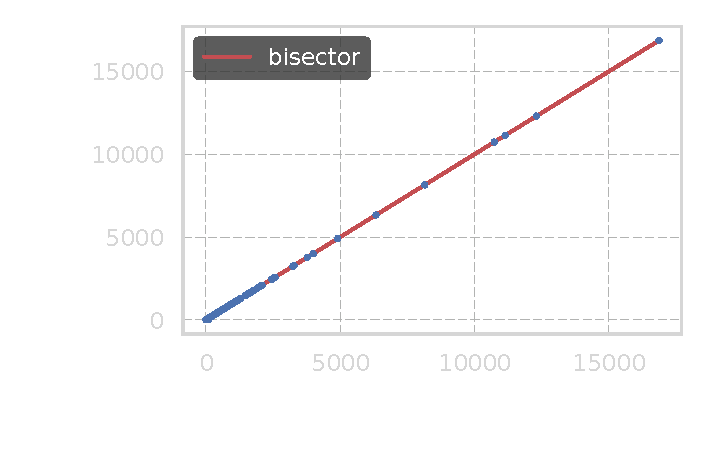
\includegraphics[width=80mm]{verif_emissions.pdf}} ;
		\visible<2->{
			\node[text centered] at (\midX,23mm) {\alert{Absence} de donnée "\alert{Weather Normalized}"} ;
		}
		\visible<3->{
			\node[text centered, text width=80mm] at (\midX,15mm) {Possiblité de \alert{calculer} à partir de la \alert{consommation totale} et des \alert{proportions d'énergies} utilisées} ;
		}
	\end{tikzpicture}
\end{frame}

\begin{frame}[t, label=ModelisationEmissions]
	\vspace{0mm}
	\begin{tikzpicture}
		\linespread{1}% <--- locally defined vertical line spacing in nodes
		\draw[clrBorders] (0,0) rectangle (\textwidth,\textheight) ;
		\nodePageNumber

		\tikzset{donnes/.style = {cyan}}

		\begin{scope}[yshift=8mm]
			\visible<2->{
			\node[box_style00, text width=30mm] (Modeles) at (0.25\textwidth,0.5\textheight) {Modèles\\"consommation"} ;
			\node[box_style00, above=of Modeles, yshift=-3mm] (Scale) {Mise à l'échelle} ;
			}
	
			\node[box_style00, donnes, above=of Scale, yshift=-3mm] (X) {$X_{train/test}$} ;
			\visible<2->{
			\draw[myarrow] (X) -- (Scale) ;
			\draw[myarrow] (Scale) -- (Modeles) ;
			}
			\visible<3->{
			\node[box_style00, right=of Modeles, xshift=0mm] (Pred) { Prediction } ;
			\node[draw, circle, right=of Pred, xshift=0mm] (logInv) { exp } ;
			\draw[myarrow] (Modeles) -- (Pred) ;
			\draw[myarrow] (Pred) -- (logInv) ;
			}
			\visible<4->{
			\node[box_style00, donnes, above=of logInv] (GFA) { $GFA_{train/test}$ } ;
			}
			\visible<5->{
			\node[draw, circle, right=of logInv] (Mult) {$\times$} ;
			\draw[myarrow] (GFA) -| (Mult) ;
			\draw[myarrow] (logInv) -- (Mult) ;
			}
	
			\visible<7->{
			\node[box_style00, below=of Mult] (CalcEmissions) {Calcul emissions} ;}
			\visible<6->{
			\node[box_style00, text width=25mm, left=of CalcEmissions] (Props) {Proportions énergies utilisées} ;
			}
			\visible<7->{
			\draw[myarrow] (Mult) -- (CalcEmissions) ;
			\draw[myarrow] (Props) -- (CalcEmissions) ;
			}
			\visible<8->{
				\node[box_style00, below=of CalcEmissions] (calcError) {Calcul de l'erreur} ;
				\node[box_style00, donnes, left=of calcError] (yTrue) {$y_{true}$} ;
				\draw[myarrow] (CalcEmissions) -- (calcError) ;
				\draw[myarrow] (yTrue) -- (calcError) ;
			}
		\end{scope}
	\end{tikzpicture}
\end{frame}



\begin{frame}[t, label=ResultsEmissions]

	% graphs: results emissions

	% meilleurs résultats pour kernel SVR rbf

	% Attention : relativement peu de données et présence d'outliers

	% \alert{REFAIRE LES CALCULS}

	\vspace{0mm}
	\begin{tikzpicture}
		\linespread{1}% <--- locally defined vertical line spacing in nodes
		\draw[clrBorders] (0,0) rectangle (\textwidth,\textheight) ;
		\nodePageNumber

		\node at (\midX,78mm) {Résultats} ;
		\node at (\midX,\midY+10mm) {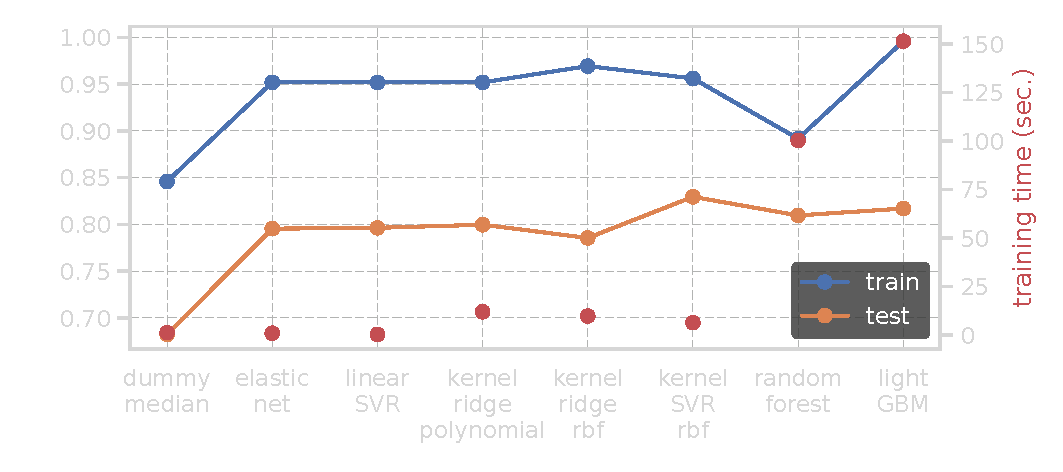
\includegraphics[width=90mm]{results_emissions.pdf}} ;

		\visible<2->{
			\node at (\midX,30mm) {Les résultats sont \alert{cohérents} avec ceux obtenus pour la consommation.} ;
		}
		\visible<3>{
			\node[text width=70mm, text centered] at (\midX,18mm) {Le modèle "\alert{kernel SVR rbf}" donne ici des\\\alert{résultats satisfaisants} pour un temps de calcul relativement court.} ;
			\begin{scope}[xshift=65.6mm, yshift=47.5mm]
				\draw[thick, rounded corners, myOrng] (0,0) rectangle (4mm, 25mm) ;
			\end{scope}
		}
	\end{tikzpicture}
\end{frame}

\section{CONCLUSION}
\begin{frame}[t, label=CCL]
	\vspace{0mm}
	\begin{tikzpicture}
		\linespread{1}% <--- locally defined vertical line spacing in nodes
		\draw[clrBorders] (0,0) rectangle (\txw,\txh) ;
		\nodePageNumber

		\node[text width=40mm, box_style00, minimum height=25mm] at (0.28\txw,63mm) {\alert{Supprimer} les \alert{10\% d'outliers} améliore les résultats.} ;

		\visible<2->{
		\node[text width=40mm, box_style00, minimum height=25mm] at (0.72\txw,63mm) {Sans les outliers, les \alert{résultats} des \alert{différents modèles} sont \alert{similaires}.} ;
		}
		\visible<3->{
		\node[text width=40mm, box_style00, minimum height=25mm] at (0.28\txw,32mm) {L'\alert{EnergySTARSCORE} est une variable \alert{pertinente} mais \alert{non essentielle} pour la prédiction de la consommation et des émissions.} ;
		}
		\visible<4->{
		\node[text width=40mm, box_style00, minimum height=25mm] at (0.72\txw,32mm) {Les \alert{émissions} peuvent être \alert{déduites} des prédictions de la \alert{consommation}. } ;
		}
	\end{tikzpicture}
\end{frame}

\section{PERSPECTIVES}
\begin{frame}[t, label=Perspectives]
	\vspace{0mm}
	\begin{tikzpicture}
		\linespread{1}% <--- locally defined vertical line spacing in nodes
		\draw[clrBorders] (0,0) rectangle (\txw,\txh) ;
		\nodePageNumber

		\node[box_style00, text width=78mm, minimum height=25mm] at (\midX,\midY+20mm) {Travailler avec un \alert{expert métier}} ;
		\visible<2->{
		\node[box_style00, text width=28mm, minimum height=25mm] (A) at (\midX-25mm,\midY-20mm) {\alert{GridsearchCV} des hyper parametres} ;
		}
		\visible<3->{
		\node[box_style00, text width=28mm, minimum height=25mm] (B) at (\midX+25mm,\midY-20mm) {\alert{Optimisation bayesienne}} ;
		\draw[myarrow] (A) -- (B) ; 
		}
	\end{tikzpicture}
\end{frame}


\begin{frame}[t, label=Merci]
	\vspace{0mm}
	\begin{tikzpicture}
		\linespread{1}% <--- locally defined vertical line spacing in nodes
		\draw[clrBorders] (0,0) rectangle (\textwidth,\textheight) ;

		\node at (0.5\textwidth,\midY) {\huge \alert{Merci} pour votre \alert{attention}.} ;

	\end{tikzpicture}
\end{frame}



\end{document}
